\section{Design and Implementation of \textsf{PCStream}}

\begin{figure}[t]
	\centering
	%\vspace{-10pt}
	%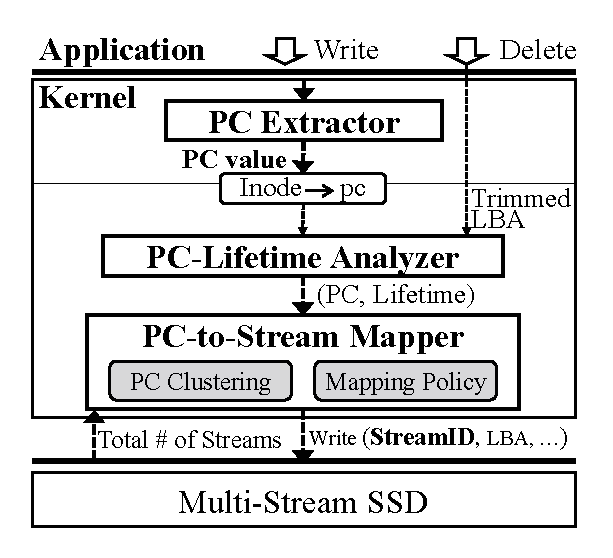
\includegraphics[width=0.6\linewidth]{figure/architecture4}
	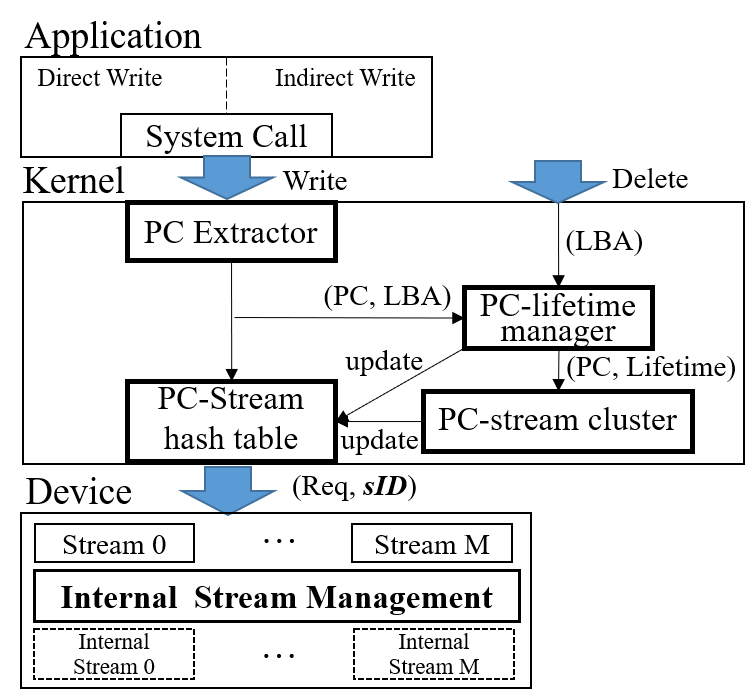
\includegraphics[width=0.8\linewidth]{figure/overview.png}
	%\vspace{-9pt}
	\caption{
		An overall architecture of \textsf{\small PCStream}. 
	}
	\label{fig:architecture}
	%\vspace{-22pt}
\end{figure}

% stream tbl (X)
% 4.2 -> 5
% short-lived app (X)
% training?

In this section, we explain the detailed implementation of \textsf{\small
PCStream}.  Fig.~\ref{fig:architecture} shows an overall architecture of
\textsf{\small PCStream}. The \textit{PC extractor module} is implemented as
part of a kernel's system call handler as already described in
Section~\ref{sec:xx}, and is responsible for computing a PC signature
from applications.  A PC signature is then delivered to the \textit{PC-lifetime
manager}, which estimates expected lifetimes of data belonging to given PCs.
Since product SSDs only expose a limited number of streams outside, the
\textit{PC-stream cluster} groups PCs with similar lifetimes using a clustering
policy, assigning PCs in a same group to an equivalent stream ID.  All the
collected information, including 1) PC signatures, 2) their expected lifetimes, and 3)
corresponding stream IDs, are maintained in the \textit{PC-stream table}.  The
information in the table is kept updated adapting to changing workloads and is
used for deciding designated stream IDs for incoming data. Finally, the
\textit{internal stream manager} implemented inside an SSD creates, removes,
and maintains internal streams stemmed from \textcolor{red}{XXX (TODO: internal stream
에 대응되는 용어가 필요할듯)}.

%the lifetime of data written by write-related system calls can be
%monitored at the program context level.  
%A PC signature value is stored in an
%inode data structure of a file system (modified for \textsf{\small PCStream})
%and is delivered to \textit{the lifetime analyzer module} which estimates
%expected lifetimes of data belonging to a given PC in the block device level.
%In order to efficiently detect the end of data lifetime in append-only
%workloads, the lifetime analyzer also intercepts TRIM~\cite{TRIM} requests from
%a file system.

%shane part Based on the lifetime information, \textit{the PC-to-stream mapper
%module} clusters PCs with similar lifetimes and maps them together to the same
%stream ID.  This mapping is required because the number of streams in an SSD
%is generally less than the number of PCs in host applications.

\subsection{PC lifetime management}
The responsibility of the PC-lifetime manager is for estimating the lifetime of
data associated with PC signatures. As mentioned before, data belonging
to a same PC signature could have slightly different lifetimes, but their
lifetime trends are almost identical, which  means that PC signatures is useful
to roughly estimate the lifetime of given data.
%, but more accurate data
%separation is required for data belonging to the same PC.  
%This issue will be discussed in Section \textcolor{red}{5.5} in detail.

\textbf{Lifetime estimation:}
In \textsf{PCStream}, the lifetime of data is defined to be an elapsed time
from when data are written until the data are invalided by TRIM commands or
overwrites. Whenever a new write request arrives that attempts to write data to
free LBAs, the PC-lifetime manager gets 1) its written time and 2) a PC
signature, along with 3) a list of LBAs, and put them into a candidate table.
Upon receiving TRIM commands or overwrite request that updates previously
written LBAs, the lifetime manager looks for a PC signature overlapped with
requested LBAs in the table and computes the lifetime (\textit{i.e.,} current
time - written time) of the corresponding PC.  The PC signature and the
expected lifetime are then put into a PC-stream table.  The written time of the
PC is replaced with the current time to keep track of future TRIM or overwrite
requests.  

Maintaining the candidate table in DRAM could be a serious burden owing to its
huge size. To mitigate this, the lifetime estimator slightly sacrifices
accuracy by increasing the granularity of LBA to 1~MB, instead of 4 KB.  The
candidate table is indexed by 1 MB LBA, and each table entry holds PC
signatures and written times. Because of coarse-grained indexing, each entry
could have multiple signatures and written times, and the same PC could span
across multiple entries.  If the same PC has different lifetimes, we take the
average one as PC's lifetime. To limit the table size, if the table reaches a
threshold size, the least recently referenced one is removed. In the current
implementation, the threshold is set to \textcolor{red}{XX MB}.

\textbf{PC-stream table:}
The PC-stream table keeps PC signatures and its expected lifetimes. To quickly
retrieve expected lifetime given a PC signature, the PC-stream table is managed
through a hash data structure. Each hash entry requires only 12 bytes: 64-bit
for a PC signature and 32-bit for an expected lifetime.  The table size is thus
quite small, such that it can be entirely loaded in DRAM. Our observations say
that the PC-stream table only consumes several tens or hundreds of KB of DRAM.

The important point that should be noted here is that the PC-stream table is
able to capture a long-term history of \textit{programs}' I/O behaviors,
regardless of their creation and deletion as the form of \textit{processes} in
the system. Thus, even for short-lived processes (\textit{e.g.,} \texttt{cpp}
and \texttt{cc1} for gcc) that are launched and terminated frequently, their
I/O behaviors are collected and applied to the PC-stream table.  This is
because PCs are unique and consistent across executions of a program.  Every PC
signature is determined by the sum of return addresses inside a process's
virtual address space.  Unless a program's binary is changed after
recompilation, those return addresses remain the same, regardless of program's
execution.  Moreover, the probability that distinct I/O activities that take
different function-call paths have the same PC signature is extremely low. This
is even true for multiple programs. Even though they are executed in the same
virtual address space, it is very unlikely that I/O activities of diverged
programs taking different function-call paths have the same PC.  We will show
this in the experimental section. Consequently, this immutable property of
the PC-stream table makes it possible for us to characterize 
unique behaviors of individual systems and workloads.

%The PC is determined by the sum of the return address, i.e., the path to reach
%the write system call.  In general, different I/O activities can not have the
%same return address because they are implemented in different functions.
%Since the probability that the sum of the different return addresses becomes
%the same is very low, the PC of an I/O activity in the same program is unique.
%For multiple programs, however, since each program uses a virtual address,
%several identical return addresses can occur.  However, the probability that
%two independent programs will have the same function call path over four or
%five is also very low, so we can usually say that a PC is unique.  Moreover,
%since the virtual address of the code is not changed after the compilation,
%the PC value will be the same when the program execution is terminated and
%restarted.  PCs of restarted program will be the same as the one of previous
%execution, and the life characteristics of the PC are also the same.  Because
%PCs are unique, if PC lifetime information is maintained, appropriate stream
%can be allocated even to the first request of a restarting program.

\subsection{Mapping PCs to SSD streams}

After estimating expected lifetimes of PC signatures, the PC-stream cluster
attempts to group PCs with similar lifetimes into an SSD stream.  This grouping
process is necessary because while product SSDs only support a limited number
of stream IDs, the number of unique PCs created is about \textcolor{red}{from 4
to 20 (너무작음)}.  For grouping, the PC-stream cluster module uses a k-means
algorithm which is lightweight and is widely used for similar purposes.  To
quickly assign a proper stream ID to incoming data, we add another field to the
PC-stream table which keeps a stream ID for each PC signature.  More
specifically, when a new write request comes, a designated SSD stream ID is
obtained by referring to the PC-stream table using request's PC value as an
index.  If there is no such a PC in the table, or a PC does not have a
designated stream ID, the request gets legacy stream ID, which is 0.

For adapting to changing workloads, re-clustering operations should be
performed regularly. This re-clustering process can be done in a
straightforward manner. The PC-stream cluster scans up-to-date lifetimes for
all PCs in the PC-stream table. Note that PC's lifetimes are updated whenever
the PC-lifetime managers gets new ones while handling write and TRIM requests,
as explained in Section 5.1.  Then, using scanned information, the PC-stream
cluster recomputes stream IDs and updates stream fields of the PC-stream table.
Scanning and recomputing require lots of CPU cycles.  To avoid significant
overhead, re-clustering is triggered when 10\% of the items in the PC-stream
table have been changed.



\begin{figure}[t]
\centering
	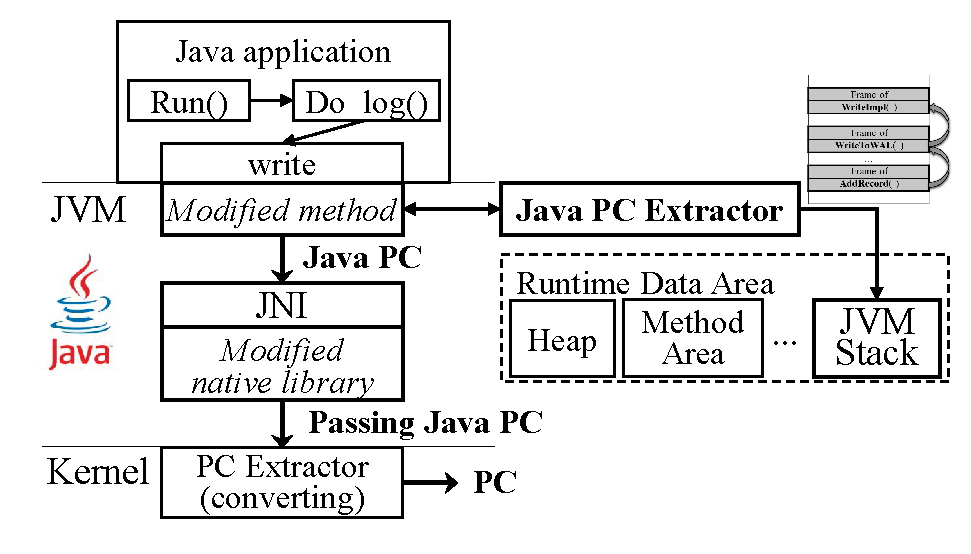
\includegraphics[width=0.6\linewidth]{figure/jvmpc}
	\caption{
	Extracting PCs for JVM \textcolor{red}{(TODO: 그림 업데이트 필요. 매우 성의
	없어 보임)} 
	}
\label{fig:java}
\end{figure}


\subsection{PC extraction for indirect writes}
One limitation of using PCs to extract I/O characteristics is that it only
works with C/C++ programs that \textit{directly} call write-related system
calls.  Many programs, however, often invoke write system calls
\textit{indirectly} through intermediate layers, which makes it difficult to
track program contexts.

The most representative example may be Java programs, such as Cassandra and
Hadoop, that run inside a Java Virtual Machine (JVM). Java programs invoke
write system calls via a native library written in C, so the PC extractor fails
to capture I/O activities because it is unable to inspect the stack of Java
processes.  Another example is a program that maintains a write buffer that is
dedicated to dealing with all the writes from other code. For example, in
MySQL~\cite{MySQL} and PostgreSQL~\cite{PostgreSQL}, every write is first
destined for a write buffer, and then flush threads materialize buffered data
to persistent storage.  In that case, the PC extractor only captures PCs of
flush threads since code that actually issues I/Os runs in other threads with
different stacks.

The problem of indirect writes can be addressed by collecting PC signatures at
the front-end interface of an intermediate layer that accepts write requests
from other parts of the program. In case of Java programs, a native library can
be modified to capture write requests and computes PC signatures. Once a native
library is modified, it automatically gathers PC signatures without modifying
application code. Fig.~\ref{fig:java} illustrates how \textsf{PCStream}
collects signatures from Java programs.  We have modified the JVM using
OpenJDK~\cite{OpenJDK} to extract PC signatures for most of write methods in
write related classes, such as \texttt{OutputStream}.  The stack area in the
\texttt{Runtime Data Areas} of JVM used to calculate PC signatures.  The
calculated PC is then passed to the write system call of the kernel via the
modified native I/O libraries.

Unlike Java, there is no a straightforward way to collect PCs from applications
with write buffers. This is because the implementation of write buffering is
different depending on applications. Thus, additional efforts to manually
modify code are unavoidable. However, the scope of this manual modification is
only limited to a write buffering code, and application logics themselves don't
need to be edited or annotated.

\subsection{Internal Stream Management}
{\color{blue}
Since it is difficult to separate data with different lifetimes within the same PC 
(as in the compaction-activity PC), we devised a two-phase method that decides SSD 
streams in two levels: the main stream in the host level and 
its internal stream in the SSD level.
Conceptually, long-lived data in the main stream are moved to its internal stream to 
separate from (future) short-lived data of the main stream.
Although moving data to the internal stream may increase WAF,
the overhead can be hidden if we restrict data copies to the internal stream during GC only.
Since long-lived data (i.e., valid pages) in a victim block are moved to a free block during GC, 
blocks belong to an internal block tend to contain long-lived data.
For instance, \textsf{\small PCStream} assigns the compaction-activity PC {\it $PC_1$} to a
main stream {\it $S_1$} in the first phase.
To separate the long-lived data of {\it $PC_1$} (e.g., L4 data) 
from future short-lived data of the same {\it $PC_1$} (e.g., L1 data), 
valid pages of the {\it $S_1$} are assigned to its internal stream for the second phase during GC.
}

%{\color{blue} 추가로, SSD가 지원하는 stream의 개수가 변경되는 상황에서도
%reclustering을 통해
%대응이 가능하다.
%reclustering의 주기는 workload의 변화 패턴에 따라 결정될 수 있다.
%새로운 PC가 계속적으로 생성되거나 한 PC의 수명 패턴이 자주 변화할 경우 reclustering의 주기를 
%좀 더 짧게 설정하여 workload 변화를 반영한다.
%}
%Since the
%number of PCs created by applications is not limited, the clustering algorithm
%must be efficient enough to quickly handle many PCs. 


